% lintrans - The linear transformation visualizer
% Copyright (C) 2021-2022 D. Dyson (DoctorDalek1963)

% This program is licensed under GNU GPLv3, available here:
% <https://www.gnu.org/licenses/gpl-3.0.html>

\documentclass[../development.tex]{subfiles}

\begin{document}

\subsubsection{Hiding the background and transformed grids\label{development:making-v0.2.2:hiding-the-background-and-transformed-grids}}

I spoke to my main stakeholder, who is the teacher that will be using \texttt{lintrans} when it's finished, and she said that the background grid and transformed grid can get a little bit in the way of the core action and make it harder to understand what's happening. Taking this feedback on board, I decided to add a display setting to toggle the background grid, and one to toggle the transformed grid.

I did the background grid first and then repeated everything for the transformed version of the grid as well. I am combining them here for brevity. The first step was of course to add a display setting for each of them. Then I had to add checkboxes for them in the display settings dialog, and then incorporate the settings into the actual drawing of the canvas.

%: d045057d568ac133b621ee9ca9daed361d570d7a
%: src/lintrans/gui/settings.py:14-27

%: d045057d568ac133b621ee9ca9daed361d570d7a
%: src/lintrans/gui/dialogs/settings.py:70,73,89-101,204,207-208,221,224-225 noscopes

%: d045057d568ac133b621ee9ca9daed361d570d7a
%: src/lintrans/gui/plots/widgets.py:60-63

%: d045057d568ac133b621ee9ca9daed361d570d7a
%: src/lintrans/gui/plots/classes.py:129-154

Then I added this change to the changelog.

%: d045057d568ac133b621ee9ca9daed361d570d7a
%: CHANGELOG.md:12-14 markdown!

\subsubsection{Hiding the basis vectors\label{development:making-v0.2.2:hiding-the-basis-vectors}}

While I was implementing new display settings, I decided to implement hiding basis vectors. This will give users the option of just seeing the grid get transformed. The process was exactly the same as before. Add the setting, add it to the dialog, use it when drawing.

%: 11ffbaf71f9fe29e1832a62f2b127aa3939e520d
%: src/lintrans/gui/settings.py:29-30

%: 11ffbaf71f9fe29e1832a62f2b127aa3939e520d
%: src/lintrans/gui/dialogs/settings.py:70,73,103-108,212,217,230,235 noscopes

%: 11ffbaf71f9fe29e1832a62f2b127aa3939e520d
%: src/lintrans/gui/plots/widgets.py:65-66

And then of course add it to the changelog.

%: 11ffbaf71f9fe29e1832a62f2b127aa3939e520d
%: CHANGELOG.md:12-14 markdown!

\subsubsection{Improving argument parsing\label{development:making-v0.2.2:improving-argument-parsing}}

Qt5 accepts arguments to its main method. I don't really know what these arguments can do, but it would be nice to be able to use them. I also want to be able to save sessions as files in the future, and it would be quite useful to open a session file by passing it as a command line argument. To make both of these easier, I decided to refactor my argument parsing.

Python has a built-in library called \pyinline{argparse}, which allows for more sophisticated argument parsing. One of the things \pyinline{argparse} can do is parse only some of the command line arguments with a method called \pyinline{parse_known_args()}\cite{argparse-parse-known-args}. I can then pass the unconsumed arguments on to Qt5. \texttt{\_\_main.py\_\_} now looks like this:

%: a688a14839caba2ee14f8551764b771ae803d935
%: src/lintrans/__main__.py

The \enquote{\pyinline{args[:1] + unparsed_args}} on line 71 means that we pass the name of the program first, and the rest of the unconsumed arguments after it.

And of course, I added it to the changelog, this time as a fix rather than an addition:

%: a688a14839caba2ee14f8551764b771ae803d935
%: CHANGELOG.md:16-18 markdown!

\subsubsection{Respecting display settings in the visual definition dialog\label{development:making-v0.2.2:respecting-display-settings-in-the-visual-definition-dialog}}

\texttt{DefineVisuallyWidget} is a subclass of \texttt{VisualizeTransformationWidget}. If it had its own instance attribute of type \pyinline{DisplaySettings}, then it could use its superclass's \pyinline{paintEvent()} method, and that would respect the display settings in the visual definition dialog.

%: 5850aa916b685992f31e58680267916927ed590d
%: src/lintrans/gui/plots/widgets.py:91-93

%: 5850aa916b685992f31e58680267916927ed590d
%: src/lintrans/gui/dialogs/define_new_matrix.py:169-180

Since the \texttt{DefineVisuallyDialog} now accepts display settings but the other definition dialogs don't, we need change the \pyinline{LintransMainWindow.dialog_define_matrix()} method to treat the visual definition dialog differently.

%: 5850aa916b685992f31e58680267916927ed590d
%: src/lintrans/gui/main_window.py:447-476

And, of course, I updated the changelog:

%: 5850aa916b685992f31e58680267916927ed590d
%: CHANGELOG.md:12,15 markdown!

\subsubsection{Changing the order in which things are drawn\label{development:making-v0.2.2:changing-the-order-in-which-things-are-drawn}}

Currently, \texttt{VisualizeTransformationWidget} draws the background, then the transformed grid, then the basis vectors, then the eigenlines and eigenvectors, then the determinant parallelogram and text. This means that the determinant parallelogram gets drawn on top of the basis vectors, which doesn't look very good. To fix this, we can simply re-order the drawing of different things. If we instead draw the transformed grid and basis vectors last, then they will appear on top of everything else, which should look significantly better.

I also renamed the \texttt{draw\_determinant\_text} display setting attribute to \texttt{show\_determinant\_value}.

Before:
%: e9da6737cbdb68e800c245bcc34e1c5c3824458a
%: src/lintrans/gui/plots/widgets.py:60-78

After:
%: acdf206a69d346dce67f74f2c54ff4c512c96229
%: src/lintrans/gui/plots/widgets.py:60-78

\begin{figure}[H]
	\hspace{0.03\linewidth}
	\begin{minipage}{0.45\linewidth}
		\begin{figure}[H]
			\centering
			\includegraphics[width=\linewidth]{development/5850aa916b685992f31e58680267916927ed590d/gui.png}
			\caption{Before re-ordering drawing commands}
			\label{fig:development:5850aa916b685992f31e58680267916927ed590d:gui.png}
		\end{figure}
	\end{minipage} \hfill
	\begin{minipage}{0.45\linewidth}
		\begin{figure}[H]
			\centering
			\includegraphics[width=\linewidth]{development/acdf206a69d346dce67f74f2c54ff4c512c96229/gui.png}
			\caption{After re-ordering drawing commands}
			\label{fig:development:acdf206a69d346dce67f74f2c54ff4c512c96229:gui.png}
		\end{figure}
	\end{minipage}
	\hspace{0.03\linewidth}
\end{figure}

\subsubsection{Improving online documentation with \textit{Read the Docs}\label{development:making-v0.2.2:improving-online-documentation-with-read-the-docs}}

So far, I've been building my documentation automatically using a tool called \texttt{Sphinx}\cite{sphinx}. I've been using it to scan through my source code, extract all the docstrings\cite{pep257-docstring-conventions}, and compile a HTML version of the source code documentation. I then publish this documentation to GitHub Pages\cite{github-pages-docs}, and all that happens automatically along with the unit tests whenever I push my changes to GitHub.

However, this system can't track changes in documentation over time. There's a popular website for hosting open source documentation, especially for Python packages, called \textit{Read the Docs}\cite{readthedocs-homepage}. It would be nice to host my documentation on there, since it would provide a standard build for the docs, and would allow me to keep track of documentation for different versions over time. I read through their tutorial and followed along with it, and then I could use Read the Docs for \texttt{lintrans}.

%: a7a8aa09148f4acf8591547d6d8b9cd8b8d52905
%: .readthedocs.yaml language=yaml

This file governs the build pipeline for the documentation. It defines how the docs will be built on the remote machine. It basically just installs all the dependencies and \texttt{lintrans} itself in a virtual environment, generates the object inventory for \texttt{intersphinx} (see \S\ref{development:preparing-for-v0.2.1:linking-in-documentation}), builds the internal import graph (see \S\ref{development:fumbling-with-semver:adding-a-graph-of-internal-imports}), and makes sure that lintrans can be installed successfully in the virtual environment. The string \enquote{\mintinline{sh}{$(pwd | sed "s/checkouts\(\/[^/]\+\)\/docs\$/envs\1/")/bin/python}} appears frequently. This string finds the version of Python that will be used for building the actual documentation at the end of the pipeline. \texttt{lintrans} has some issues with circular imports, which means that it can only be installed in editable mode\footnote{Editable mode is an option that you can choose when installing a package with \texttt{pip}\cite{pip-install-editable}. Instead of copying the source code to the installation directory like normal, it creates a link to the source code from the installation directory - basically a symlink in Linux. This means that if you change the source code, the installed version gets updated instantly, which is obviously very useful for fast, iterative development. It also has some strange effects with import order and resolution. Importing packages and modules is very complicated in Python\cite{david-beazley-python-modules}, and I repeatedly failed to get \texttt{lintrans} to be installable without editable mode, so I had to resort to just using this bodge on Read the Docs instead.}. This means that I have to bodge the build system to install \texttt{lintrans} properly.

Additionally, having a build system like this means that builds should be repeatable, which means I should pin the exact versions of all my dependencies, to avoid any breaking changes in the future.

%: 152f9e59b5b4e22607cf2b687c85c70708054579
%: requirements.txt language="lexers.py:CommentedTextLexer -x"

%: 152f9e59b5b4e22607cf2b687c85c70708054579
%: dev_requirements.txt language="lexers.py:CommentedTextLexer -x"

%: 152f9e59b5b4e22607cf2b687c85c70708054579
%: docs/docs_requirements.txt language="lexers.py:CommentedTextLexer -x"

Now that I was using Read the Docs, I could remove the old GitHub Actions workflow to compile the documentation.

\subsubsection{Parsing parentheses\label{development:making-v0.2.2:parsing-parentheses}}

\texttt{git} has a feature called branches\cite{git-docs-branch}, which allow you to work on different things simultaneously. A branch is basically a sandbox where you can make changes and focus on a particular feature while not having to worry about the rest of the project. It's particularly good for teams where different people can work on different features at the same time, but it's also useful for individual developers. The first feature branch I merged for \texttt{lintrans} was called \texttt{dev/parse-parens}. I created it a week or two ago, and I used it to focus on improving the parser to understand parenthesised expressions like \pyinline{"A(B+C)^2"}.

\paragraph{Extending validation\label{development:making-v0.2.2:parsing-parentheses:extending-validation}}

The first thing I needed to do was allow parenthesised expressions as valid. If the validator rejects them, then they can never be parsed. Any expression can be evaluated to a matrix, and a pair of balanced parentheses can contain any valid expression. As such, a parenthesised expression can be considered as a type of matrix.

%: 1e49c1479939b8de04751ab1a798afb2145b1550
%: docs/source/bnf.txt language="lexers.py:BnfHashtagCommentLexer -x"

%: 1e49c1479939b8de04751ab1a798afb2145b1550
%: src/lintrans/matrices/parse.py:16,23-118

We create a naïve character class that just contains all characters that could possibly be in a valid expression. Then when we compile the naïve expression pattern, we say that a matrix identifier can be one of three things: it can be a capital letter, the \texttt{rot()} command with a real number angle, or a balanced pair of parentheses around some characters. The characters in the parentheses are not validated at this stage (hence why this pattern is naïve), but we know that those characters are only allowed to be from the naïve character class.

Then we have a function that finds sub-expressions in a given expression. It simply scans through the given string with a pointer and keeps track of the current sub-expression. It uses the \pyinline{paren_depth} variable to keep track of how deep into a sub-expression it currently is. This function deliberately avoids counting the parentheses from \texttt{rot()} commands towards the \pyinline{paren_depth}. This is to avoid scanning an expression like \pyinline{"3rot(45)^2"} and finding \pyinline{"45"} as a sub-expression.

Then we have to actually use this function when validating. All we do is recursively check that each sub-expression is a valid expression on its own. The \pyinline{find_sub_expressions()} function only goes one level deep, so in an expression like \pyinline{"A(B+C(D^2-E))"}, it will only find \pyinline{"B+C(D^2-E)"} as a sub-expression, so recursion is needed to make the validation work properly.

There's actually a small mistake in the BNF that I didn't notice until much much later. The validation code is correct - it treats a parenthesised expression as a matrix identifier, so it can accept a multiplier on the left and an index on the right - but the BNF treats a parenthesised expression as a full matrix, which means it can't accept a multiplier or index. This doesn't affect the code, but does make the documentation slightly confusing.

And of course, I then added to the automatic unit tests to make sure this new validation worked.

%: 1e49c1479939b8de04751ab1a798afb2145b1550
%: tests/matrices/test_parse_and_validate_expression.py:16-30,33,50-52,54,57,60,70,105-111

I also added \pyinline{@pytest.mark.xfail} to \pyinline{test_parse_matrix_expression()}, since parsing should fail with the parenthesised expressions because I haven't implemented it yet.

\pytestScreenshot{1e49c1479939b8de04751ab1a798afb2145b1550}

\paragraph{Creating the parser class\label{development:making-v0.2.2:parsing-parentheses:creating-the-parser-class}}

I previously used regular expressions to parse matrix expressions. The algorithm would replace various parts of the expression to coerce it into the correct format, and then use a big RegEx at the end to find all the parts necessary for parsing. This was hard to understand and hard to maintain. It's now time to overhaul this parsing system and use a parser class to scan through the input and parse character-by-character, keeping track of the state as it goes.

%: 736809714e0ad7579c419db03c4b5d8b8fd0c1a1
%: src/lintrans/matrices/parse.py:122-351

The \pyinline{MatrixToken} class just holds data about a matrix multiplier, identifier, and exponent. It's just a simple way to package up this data into a single dataclass to keep track of which matrices we've parsed.

The \pyinline{ExpressionParser} class works like so: when you create a new instance, you give it an expression to parse and it cleans up the expression by removing whitespace, making sure it's valid, wrapping exponents with \texttt{\{\}}, etc. Most of these replacement steps are taken from the previous RegEx-based parser. It then sets up some internal state to keep track of the expression, the pointer, the token that it's currently parsing, the group that it's currently parsing, and its progress so far.

When you've created a new instance, you should call the public \pyinline{parse()} method, which will return the parsed expression at the end, in the same format that the old parser used. The \pyinline{parse_matrix_expression()} function is a wrapper that just creates an \pyinline{ExpressionParser} and calls \pyinline{parse()}.

The \pyinline{parse()} method itself just delegates to \pyinline{_parse_multiplication_group()}. A multiplication group is a group of matrices that will be multiplied together in a particular order. An expression should start with a multiplication group, and may have extra ones separated with plus signs. When all the multiplication groups have been parsed, it returns the final parse list.

\pyinline{_parse_multiplication_group()} tries to parse matrices until it reaches the end of the expression or it finds a plus sign, at which point it appends the current group to the final list and returns.

\pyinline{_parse_matrix()} returns a boolean to indicate success. It just attempts to parse a \enquote{matrix part} (multiplier, identifier, or exponent) until that fails, and then ensures that the resultant matrix token has a valid identifier. It then appends the matrix token to the current group.

\pyinline{_parse_matrix_part()} is where most of the selection happens. This method has to determine if it's looking at a multiplier, which would start with a digit or a minus sign; a normal identifier, which would start with a capital letter; a rotation identifier, which would start with a lowercase letter r; a sub-expression, which would start with an open bracket; or an exponent, with will start with a caret. If it encounters a plus sign, then that's a soft error, so it can return \pyinline{False}, but if it encounters something it doesn't recognise, then that's a hard error.

\pyinline{_parse_multiplier()} just parses a real number into \pyinline{self.current_token.multiplier}.

\pyinline{_parse_rot_identifier()} parses a \texttt{rot()} command with a real number angle\footnote{It doesn't need to parse the real number itself to make sure it's valid, since the expression validator already ensured that it was a valid real number.}.

\pyinline{_parse_sub_expression()} hasn't been implemented yet, but it will eventually parse sub-expressions, hence the name.

\pyinline{_parse_exponent()} parses a caret, and then a balanced pair of braces, containing an integer or a capital letter T.

And of course, this new parser should still pass all the unit tests for the previous parser, which it does.

% The tests haven't changed at all, so we can just use the previous image
\pytestScreenshot{1e49c1479939b8de04751ab1a798afb2145b1550}

\paragraph{Implementing sub-expression parsing\label{development:making-v0.2.2:parsing-parentheses:implementing-sub-expression-parsing}}

Of course, the next step was to actually implement sub-expression parsing. To do this, I used a very similar method to finding the sub-expressions, where I kept track of the depth of the parentheses. Except with this method, we only wanted the first sub-expression starting at the pointer. We can then assign this whole sub-expression to \pyinline{self.current_token.identifier} at the end.

Much like when finding sub-expressions, this parser method only goes one level deep, but the \pyinline{MatrixWrapper} will use recursion when evaluating the parsed expressions, so it will handle nested sub-expressions with.

%: 493f8cf3fb658408466f099f978d276fc2262243
%: src/lintrans/matrices/parse.py:305-332

\paragraph{Fixing little bugs\label{development:making-v0.2.2:parsing-parentheses:fixing-little-bugs}}

Since I've now implemented sub-expression parsing, I should be able to just remove the \pyinline{@pytest.mark.xfail} line from before and all the tests should pass with no problem.

\pytestScreenshot[One of the tests failing]{493f8cf3fb658408466f099f978d276fc2262243-noxfail}

Ah. That's not good. So what went wrong? Well, we can see from the output that \pyinline{test_parse_matrix_expression()} is the one that failed. This test iterates over a whole list, so which element broke it? Well, we can see from the line \enquote{\pyinline{self = lintrans.matrices.parse.ExpressionParser(".1A")}} that it was trying to parse the expression \pyinline{".1A"}. This doesn't work, not because \pyinline{ExpressionParser._parse_multiplier()} doesn't understand this type of multiplier, but because \pyinline{ExpressionParser._parse_matrix_part()} doesn't recognise a dot as the start of a multiplier, so never calls \pyinline{_parse_multiplier()}. This would be a very easy fix, but this error got me thinking about these multipliers and I decided to just forbid them. They can create confusion; \pyinline{"0.1A"} is easier to understand than \pyinline{".1A"}. Implementing this change just meant removing this type of multiplier from the tests.

Once I'd done that, the parser should work fine, right?

\pytestScreenshot[Another test failing]{9b1c69926c225574161d32dcbecd86055edb4065-noxfail}

Well, that's strange. It was trying to parse the expression \pyinline{"A 0.1B"} but it thought the \texttt{0.1} was part of the \texttt{A}. Why did that happen? Well, it's because of line 232 in this snippet:

%: 9b1c69926c225574161d32dcbecd86055edb4065
%: src/lintrans/matrices/parse.py:231-235

The parser parsed \pyinline{"A"} as the matrix identifier and then encountered \pyinline{"0"}. Since the current token didn't have a multiplier, it started parsing a multiplier for the matrix $\mathbf{A}$. To fix this, we can just fail to parse a matrix part if we encounter the start of a multiplier when the current token already has an identifier. Failing to parse a matrix part here means that the parser will start parsing a new matrix.

%: 8d7143fc33ea7bd4199e0f01b6a5308dfcf03ff9
%: src/lintrans/matrices/parse.py:231-236

That should fix the tests, right?

\pytestScreenshot[\textit{Another} test failing]{9b1c69926c225574161d32dcbecd86055edb4065-noxfail-fixed-mul-order}

I'm getting tired of this now. What's broken this time? Well, the parser processes its input to remove whitespace and add braces around exponents before any parsing takes place. This includes processing the contents of sub-expressions. That was never a problem before, since parsing wasn't affected by whitespace or braces, but now those changes propagate into the sub-expressions. I wrote the sub-expression parsing tests in \S\ref{development:making-v0.2.2:parsing-parentheses:extending-validation} by using my literal expression input in the parsed sub-expressions. So to fix this error, I just had to account for the syntax transformations in the test input.

\textit{Now} the tests should all pass, right?

\pytestScreenshot[All the tests finally passing]{8d7143fc33ea7bd4199e0f01b6a5308dfcf03ff9}

Thank god.

\end{document}
